\documentclass[1p]{elsarticle_modified}
%\bibliographystyle{elsarticle-num}

%\usepackage[colorlinks]{hyperref}
%\usepackage{abbrmath_seonhwa} %\Abb, \Ascr, \Acal ,\Abf, \Afrak
\usepackage{amsfonts}
\usepackage{amssymb}
\usepackage{amsmath}
\usepackage{amsthm}
\usepackage{scalefnt}
\usepackage{amsbsy}
\usepackage{kotex}
\usepackage{caption}
\usepackage{subfig}
\usepackage{color}
\usepackage{graphicx}
\usepackage{xcolor} %% white, black, red, green, blue, cyan, magenta, yellow
\usepackage{float}
\usepackage{setspace}
\usepackage{hyperref}

\usepackage{tikz}
\usetikzlibrary{arrows}

\usepackage{multirow}
\usepackage{array} % fixed length table
\usepackage{hhline}

%%%%%%%%%%%%%%%%%%%%%
\makeatletter
\renewcommand*\env@matrix[1][\arraystretch]{%
	\edef\arraystretch{#1}%
	\hskip -\arraycolsep
	\let\@ifnextchar\new@ifnextchar
	\array{*\c@MaxMatrixCols c}}
\makeatother %https://tex.stackexchange.com/questions/14071/how-can-i-increase-the-line-spacing-in-a-matrix
%%%%%%%%%%%%%%%

\usepackage[normalem]{ulem}

\newcommand{\msout}[1]{\ifmmode\text{\sout{\ensuremath{#1}}}\else\sout{#1}\fi}
%SOURCE: \msout is \stkout macro in https://tex.stackexchange.com/questions/20609/strikeout-in-math-mode

\newcommand{\cancel}[1]{
	\ifmmode
	{\color{red}\msout{#1}}
	\else
	{\color{red}\sout{#1}}
	\fi
}

\newcommand{\add}[1]{
	{\color{blue}\uwave{#1}}
}

\newcommand{\replace}[2]{
	\ifmmode
	{\color{red}\msout{#1}}{\color{blue}\uwave{#2}}
	\else
	{\color{red}\sout{#1}}{\color{blue}\uwave{#2}}
	\fi
}

\newcommand{\Sol}{\mathcal{S}} %segment
\newcommand{\D}{D} %diagram
\newcommand{\A}{\mathcal{A}} %arc


%%%%%%%%%%%%%%%%%%%%%%%%%%%%%5 test

\def\sl{\operatorname{\textup{SL}}(2,\Cbb)}
\def\psl{\operatorname{\textup{PSL}}(2,\Cbb)}
\def\quan{\mkern 1mu \triangleright \mkern 1mu}

\theoremstyle{definition}
\newtheorem{thm}{Theorem}[section]
\newtheorem{prop}[thm]{Proposition}
\newtheorem{lem}[thm]{Lemma}
\newtheorem{ques}[thm]{Question}
\newtheorem{cor}[thm]{Corollary}
\newtheorem{defn}[thm]{Definition}
\newtheorem{exam}[thm]{Example}
\newtheorem{rmk}[thm]{Remark}
\newtheorem{alg}[thm]{Algorithm}

\newcommand{\I}{\sqrt{-1}}
\begin{document}

%\begin{frontmatter}
%
%\title{Boundary parabolic representations of knots up to 8 crossings}
%
%%% Group authors per affiliation:
%\author{Yunhi Cho} 
%\address{Department of Mathematics, University of Seoul, Seoul, Korea}
%\ead{yhcho@uos.ac.kr}
%
%
%\author{Seonhwa Kim} %\fnref{s_kim}}
%\address{Center for Geometry and Physics, Institute for Basic Science, Pohang, 37673, Korea}
%\ead{ryeona17@ibs.re.kr}
%
%\author{Hyuk Kim}
%\address{Department of Mathematical Sciences, Seoul National University, Seoul 08826, Korea}
%\ead{hyukkim@snu.ac.kr}
%
%\author{Seokbeom Yoon}
%\address{Department of Mathematical Sciences, Seoul National University, Seoul, 08826,  Korea}
%\ead{sbyoon15@snu.ac.kr}
%
%\begin{abstract}
%We find all boundary parabolic representation of knots up to 8 crossings.
%
%\end{abstract}
%\begin{keyword}
%    \MSC[2010] 57M25 
%\end{keyword}
%
%\end{frontmatter}

%\linenumbers
%\tableofcontents
%
\newcommand\colored[1]{\textcolor{white}{\rule[-0.35ex]{0.8em}{1.4ex}}\kern-0.8em\color{red} #1}%
%\newcommand\colored[1]{\textcolor{white}{ #1}\kern-2.17ex	\textcolor{white}{ #1}\kern-1.81ex	\textcolor{white}{ #1}\kern-2.15ex\color{red}#1	}

{\Large $\underline{11a_{319}~(K11a_{319})}$}

\setlength{\tabcolsep}{10pt}
\renewcommand{\arraystretch}{1.6}
\vspace{1cm}\begin{tabular}{m{100pt}>{\centering\arraybackslash}m{274pt}}
\multirow{5}{120pt}{
	\centering
	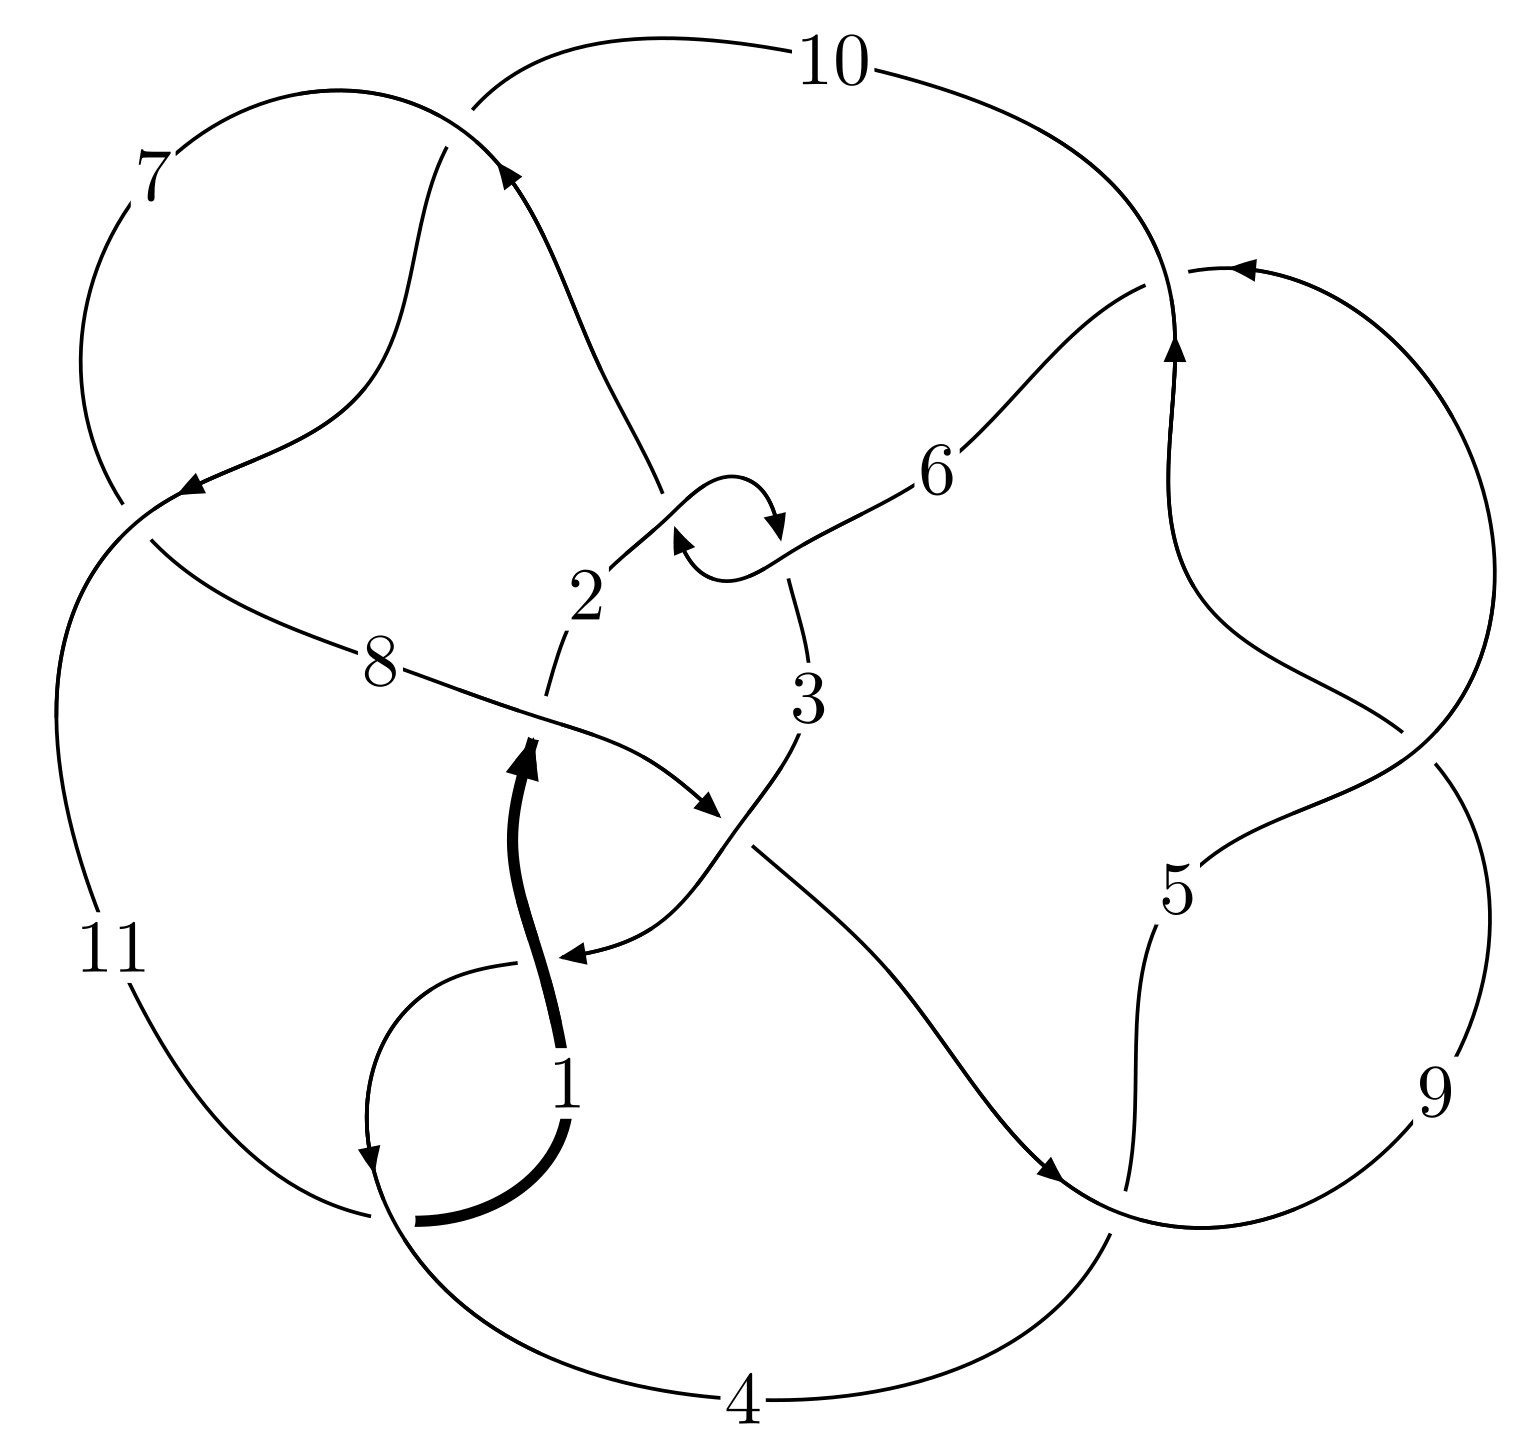
\includegraphics[width=112pt]{../../../GIT/diagram.site/Diagrams/png/568_11a_319.png}\\
\ \ \ A knot diagram\footnotemark}&
\allowdisplaybreaks
\textbf{Linearized knot diagam} \\
\cline{2-2}
 &
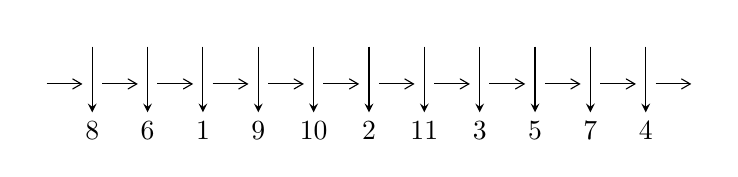
\begin{tikzpicture}[x=20pt, y=17pt]
	% nodes
	\node (C0) at (0, 0) {};
	\node (C1) at (1, 0) {};
	\node (C1U) at (1, +1) {};
	\node (C1D) at (1, -1) {8};

	\node (C2) at (2, 0) {};
	\node (C2U) at (2, +1) {};
	\node (C2D) at (2, -1) {6};

	\node (C3) at (3, 0) {};
	\node (C3U) at (3, +1) {};
	\node (C3D) at (3, -1) {1};

	\node (C4) at (4, 0) {};
	\node (C4U) at (4, +1) {};
	\node (C4D) at (4, -1) {9};

	\node (C5) at (5, 0) {};
	\node (C5U) at (5, +1) {};
	\node (C5D) at (5, -1) {10};

	\node (C6) at (6, 0) {};
	\node (C6U) at (6, +1) {};
	\node (C6D) at (6, -1) {2};

	\node (C7) at (7, 0) {};
	\node (C7U) at (7, +1) {};
	\node (C7D) at (7, -1) {11};

	\node (C8) at (8, 0) {};
	\node (C8U) at (8, +1) {};
	\node (C8D) at (8, -1) {3};

	\node (C9) at (9, 0) {};
	\node (C9U) at (9, +1) {};
	\node (C9D) at (9, -1) {5};

	\node (C10) at (10, 0) {};
	\node (C10U) at (10, +1) {};
	\node (C10D) at (10, -1) {7};

	\node (C11) at (11, 0) {};
	\node (C11U) at (11, +1) {};
	\node (C11D) at (11, -1) {4};
	\node (C12) at (12, 0) {};

	% arrows
	\draw[->,>={angle 60}]
	(C0) edge (C1) (C1) edge (C2) (C2) edge (C3) (C3) edge (C4) (C4) edge (C5) (C5) edge (C6) (C6) edge (C7) (C7) edge (C8) (C8) edge (C9) (C9) edge (C10) (C10) edge (C11) (C11) edge (C12) ;	\draw[->,>=stealth]
	(C1U) edge (C1D) (C2U) edge (C2D) (C3U) edge (C3D) (C4U) edge (C4D) (C5U) edge (C5D) (C6U) edge (C6D) (C7U) edge (C7D) (C8U) edge (C8D) (C9U) edge (C9D) (C10U) edge (C10D) (C11U) edge (C11D) ;
	\end{tikzpicture} \\
\hhline{~~} \\& 
\textbf{Solving Sequence} \\ \cline{2-2} 
 &
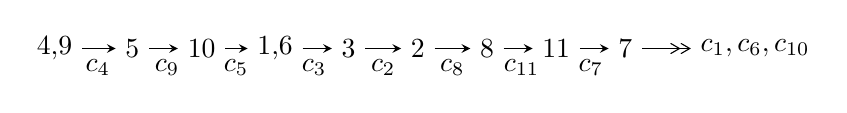
\begin{tikzpicture}[x=25pt, y=7pt]
	% node
	\node (A0) at (-1/8, 0) {4,9};
	\node (A1) at (1, 0) {5};
	\node (A2) at (2, 0) {10};
	\node (A3) at (49/16, 0) {1,6};
	\node (A4) at (33/8, 0) {3};
	\node (A5) at (41/8, 0) {2};
	\node (A6) at (49/8, 0) {8};
	\node (A7) at (57/8, 0) {11};
	\node (A8) at (65/8, 0) {7};
	\node (C1) at (1/2, -1) {$c_{4}$};
	\node (C2) at (3/2, -1) {$c_{9}$};
	\node (C3) at (5/2, -1) {$c_{5}$};
	\node (C4) at (29/8, -1) {$c_{3}$};
	\node (C5) at (37/8, -1) {$c_{2}$};
	\node (C6) at (45/8, -1) {$c_{8}$};
	\node (C7) at (53/8, -1) {$c_{11}$};
	\node (C8) at (61/8, -1) {$c_{7}$};
	\node (A9) at (10, 0) {$c_{1},c_{6},c_{10}$};

	% edge
	\draw[->,>=stealth]	
	(A0) edge (A1) (A1) edge (A2) (A2) edge (A3) (A3) edge (A4) (A4) edge (A5) (A5) edge (A6) (A6) edge (A7) (A7) edge (A8) ;
	\draw[->>,>={angle 60}]	
	(A8) edge (A9);
\end{tikzpicture} \\ 

\end{tabular} \\

\footnotetext{
The image of knot diagram is generated by the software ``\textbf{Draw programme}" developed by Andrew Bartholomew(\url{http://www.layer8.co.uk/maths/draw/index.htm\#Running-draw}), where we modified some parts for our purpose(\url{https://github.com/CATsTAILs/LinksPainter}).
}\phantom \\ \newline 
\centering \textbf{Ideals for irreducible components\footnotemark of $X_{\text{par}}$} 
 
\begin{align*}
I^u_{1}&=\langle 
-3.02320\times10^{126} u^{75}-1.11777\times10^{126} u^{74}+\cdots+3.99495\times10^{125} b-2.42597\times10^{127},\\
\phantom{I^u_{1}}&\phantom{= \langle  }-1.55725\times10^{127} u^{75}-6.75726\times10^{126} u^{74}+\cdots+4.39445\times10^{126} a-1.20832\times10^{128},\\
\phantom{I^u_{1}}&\phantom{= \langle  }u^{76}- u^{75}+\cdots+20 u-11\rangle \\
I^u_{2}&=\langle 
u^{14}-8 u^{12}+2 u^{11}+24 u^{10}-12 u^9-31 u^8+25 u^7+12 u^6-20 u^5+6 u^4+4 u^3-4 u^2+b+u+1,\\
\phantom{I^u_{2}}&\phantom{= \langle  }u^7-5 u^5+u^4+7 u^3-3 u^2+a-2 u+2,\;u^{17}-10 u^{15}+\cdots-4 u+1\rangle \\
\\
\end{align*}
\raggedright * 2 irreducible components of $\dim_{\mathbb{C}}=0$, with total 93 representations.\\
\footnotetext{All coefficients of polynomials are rational numbers. But the coefficients are sometimes approximated in decimal forms when there is not enough margin.}
\newpage
\renewcommand{\arraystretch}{1}
\centering \section*{I. $I^u_{1}= \langle -3.02\times10^{126} u^{75}-1.12\times10^{126} u^{74}+\cdots+3.99\times10^{125} b-2.43\times10^{127},\;-1.56\times10^{127} u^{75}-6.76\times10^{126} u^{74}+\cdots+4.39\times10^{126} a-1.21\times10^{128},\;u^{76}- u^{75}+\cdots+20 u-11 \rangle$}
\flushleft \textbf{(i) Arc colorings}\\
\begin{tabular}{m{7pt} m{180pt} m{7pt} m{180pt} }
\flushright $a_{4}=$&$\begin{pmatrix}1\\0\end{pmatrix}$ \\
\flushright $a_{9}=$&$\begin{pmatrix}0\\u\end{pmatrix}$ \\
\flushright $a_{5}=$&$\begin{pmatrix}1\\u^2\end{pmatrix}$ \\
\flushright $a_{10}=$&$\begin{pmatrix}- u\\- u^3+u\end{pmatrix}$ \\
\flushright $a_{1}=$&$\begin{pmatrix}3.54367 u^{75}+1.53768 u^{74}+\cdots-35.9783 u+27.4965\\7.56756 u^{75}+2.79795 u^{74}+\cdots-67.2178 u+60.7258\end{pmatrix}$ \\
\flushright $a_{6}=$&$\begin{pmatrix}- u^2+1\\- u^4+2 u^2\end{pmatrix}$ \\
\flushright $a_{3}=$&$\begin{pmatrix}-5.63330 u^{75}-2.05372 u^{74}+\cdots+46.7663 u-43.7933\\-1.63145 u^{75}-0.0719719 u^{74}+\cdots+15.8051 u-16.2500\end{pmatrix}$ \\
\flushright $a_{2}=$&$\begin{pmatrix}-6.48406 u^{75}-2.02652 u^{74}+\cdots+54.0242 u-53.0924\\0.680076 u^{75}+0.626654 u^{74}+\cdots-5.15979 u+3.31366\end{pmatrix}$ \\
\flushright $a_{8}=$&$\begin{pmatrix}-5.69380 u^{75}-2.66010 u^{74}+\cdots+46.9149 u-40.6325\\-5.61367 u^{75}-2.27578 u^{74}+\cdots+50.6262 u-43.0534\end{pmatrix}$ \\
\flushright $a_{11}=$&$\begin{pmatrix}11.1112 u^{75}+4.33563 u^{74}+\cdots-103.196 u+88.2222\\7.56756 u^{75}+2.79795 u^{74}+\cdots-67.2178 u+60.7258\end{pmatrix}$ \\
\flushright $a_{7}=$&$\begin{pmatrix}-12.8280 u^{75}-5.10092 u^{74}+\cdots+116.740 u-101.789\\-9.74429 u^{75}-3.51162 u^{74}+\cdots+86.7191 u-78.0492\end{pmatrix}$\\ \flushright $a_{7}=$&$\begin{pmatrix}-12.8280 u^{75}-5.10092 u^{74}+\cdots+116.740 u-101.789\\-9.74429 u^{75}-3.51162 u^{74}+\cdots+86.7191 u-78.0492\end{pmatrix}$\\&\end{tabular}
\flushleft \textbf{(ii) Obstruction class $= -1$}\\~\\
\flushleft \textbf{(iii) Cusp Shapes $= 17.3913 u^{75}+5.44974 u^{74}+\cdots-141.033 u+132.140$}\\~\\
\newpage\renewcommand{\arraystretch}{1}
\flushleft \textbf{(iv) u-Polynomials at the component}\newline \\
\begin{tabular}{m{50pt}|m{274pt}}
Crossings & \hspace{64pt}u-Polynomials at each crossing \\
\hline $$\begin{aligned}c_{1}\end{aligned}$$&$\begin{aligned}
&u^{76}- u^{75}+\cdots+412 u-8
\end{aligned}$\\
\hline $$\begin{aligned}c_{2},c_{6}\end{aligned}$$&$\begin{aligned}
&u^{76}+2 u^{75}+\cdots-3 u-1
\end{aligned}$\\
\hline $$\begin{aligned}c_{3},c_{11}\end{aligned}$$&$\begin{aligned}
&u^{76}-2 u^{75}+\cdots-9 u+1
\end{aligned}$\\
\hline $$\begin{aligned}c_{4},c_{5},c_{9}\end{aligned}$$&$\begin{aligned}
&u^{76}- u^{75}+\cdots+20 u-11
\end{aligned}$\\
\hline $$\begin{aligned}c_{7},c_{10}\end{aligned}$$&$\begin{aligned}
&u^{76}-27 u^{74}+\cdots+87 u+89
\end{aligned}$\\
\hline $$\begin{aligned}c_{8}\end{aligned}$$&$\begin{aligned}
&u^{76}+u^{75}+\cdots-656 u-71
\end{aligned}$\\
\hline
\end{tabular}\\~\\
\newpage\renewcommand{\arraystretch}{1}
\flushleft \textbf{(v) Riley Polynomials at the component}\newline \\
\begin{tabular}{m{50pt}|m{274pt}}
Crossings & \hspace{64pt}Riley Polynomials at each crossing \\
\hline $$\begin{aligned}c_{1}\end{aligned}$$&$\begin{aligned}
&y^{76}+7 y^{75}+\cdots-193744 y+64
\end{aligned}$\\
\hline $$\begin{aligned}c_{2},c_{6}\end{aligned}$$&$\begin{aligned}
&y^{76}+38 y^{75}+\cdots+9 y+1
\end{aligned}$\\
\hline $$\begin{aligned}c_{3},c_{11}\end{aligned}$$&$\begin{aligned}
&y^{76}+38 y^{75}+\cdots-35 y+1
\end{aligned}$\\
\hline $$\begin{aligned}c_{4},c_{5},c_{9}\end{aligned}$$&$\begin{aligned}
&y^{76}-77 y^{75}+\cdots-1918 y+121
\end{aligned}$\\
\hline $$\begin{aligned}c_{7},c_{10}\end{aligned}$$&$\begin{aligned}
&y^{76}-54 y^{75}+\cdots-315687 y+7921
\end{aligned}$\\
\hline $$\begin{aligned}c_{8}\end{aligned}$$&$\begin{aligned}
&y^{76}+3 y^{75}+\cdots+35282 y+5041
\end{aligned}$\\
\hline
\end{tabular}\\~\\
\newpage\flushleft \textbf{(vi) Complex Volumes and Cusp Shapes}
$$\begin{array}{c|c|c}  
\text{Solutions to }I^u_{1}& \I (\text{vol} + \sqrt{-1}CS) & \text{Cusp shape}\\
 \hline 
\begin{aligned}
u &= \phantom{-}0.389612 + 0.916154 I \\
a &= \phantom{-}0.592515 - 1.155730 I \\
b &= -0.401944 + 1.052230 I\end{aligned}
 & \phantom{-}0.62066 + 1.50555 I & \phantom{-0.000000 } 0 \\ \hline\begin{aligned}
u &= \phantom{-}0.389612 - 0.916154 I \\
a &= \phantom{-}0.592515 + 1.155730 I \\
b &= -0.401944 - 1.052230 I\end{aligned}
 & \phantom{-}0.62066 - 1.50555 I & \phantom{-0.000000 } 0 \\ \hline\begin{aligned}
u &= \phantom{-}0.823395 + 0.409350 I \\
a &= -1.05402 + 1.27829 I \\
b &= \phantom{-}0.263172 - 0.984227 I\end{aligned}
 & \phantom{-}4.83635 + 1.37448 I & \phantom{-0.000000 } 0 \\ \hline\begin{aligned}
u &= \phantom{-}0.823395 - 0.409350 I \\
a &= -1.05402 - 1.27829 I \\
b &= \phantom{-}0.263172 + 0.984227 I\end{aligned}
 & \phantom{-}4.83635 - 1.37448 I & \phantom{-0.000000 } 0 \\ \hline\begin{aligned}
u &= -0.483501 + 0.974155 I \\
a &= \phantom{-}0.45679 + 1.67940 I \\
b &= \phantom{-}0.550419 - 1.214740 I\end{aligned}
 & \phantom{-}2.29106 + 11.42070 I & \phantom{-0.000000 } 0 \\ \hline\begin{aligned}
u &= -0.483501 - 0.974155 I \\
a &= \phantom{-}0.45679 - 1.67940 I \\
b &= \phantom{-}0.550419 + 1.214740 I\end{aligned}
 & \phantom{-}2.29106 - 11.42070 I & \phantom{-0.000000 } 0 \\ \hline\begin{aligned}
u &= -0.424777 + 0.743415 I \\
a &= -0.237044 - 0.126527 I \\
b &= \phantom{-}0.926094 + 0.184524 I\end{aligned}
 & -0.84401 + 6.11908 I & -11.00000 - 6.39496 I \\ \hline\begin{aligned}
u &= -0.424777 - 0.743415 I \\
a &= -0.237044 + 0.126527 I \\
b &= \phantom{-}0.926094 - 0.184524 I\end{aligned}
 & -0.84401 - 6.11908 I & -11.00000 + 6.39496 I \\ \hline\begin{aligned}
u &= -0.814292 + 0.244342 I \\
a &= \phantom{-}1.026810 + 0.480678 I \\
b &= \phantom{-}0.092563 - 0.921471 I\end{aligned}
 & -0.099237 + 0.900566 I & -11.00000 + 0. I\phantom{ +0.000000I} \\ \hline\begin{aligned}
u &= -0.814292 - 0.244342 I \\
a &= \phantom{-}1.026810 - 0.480678 I \\
b &= \phantom{-}0.092563 + 0.921471 I\end{aligned}
 & -0.099237 - 0.900566 I & -11.00000 + 0. I\phantom{ +0.000000I}\\
 \hline 
 \end{array}$$\newpage$$\begin{array}{c|c|c}  
\text{Solutions to }I^u_{1}& \I (\text{vol} + \sqrt{-1}CS) & \text{Cusp shape}\\
 \hline 
\begin{aligned}
u &= -0.176061 + 0.818582 I \\
a &= \phantom{-}0.40528 + 1.71607 I \\
b &= -0.156652 - 0.429229 I\end{aligned}
 & -1.33166 - 1.72547 I & -14.8473 + 4.3130 I \\ \hline\begin{aligned}
u &= -0.176061 - 0.818582 I \\
a &= \phantom{-}0.40528 - 1.71607 I \\
b &= -0.156652 + 0.429229 I\end{aligned}
 & -1.33166 + 1.72547 I & -14.8473 - 4.3130 I \\ \hline\begin{aligned}
u &= \phantom{-}0.543220 + 0.596118 I \\
a &= -0.72897 + 1.68729 I \\
b &= -0.578793 - 1.217190 I\end{aligned}
 & -0.40362 - 6.16038 I & -12.6367 + 6.4189 I \\ \hline\begin{aligned}
u &= \phantom{-}0.543220 - 0.596118 I \\
a &= -0.72897 - 1.68729 I \\
b &= -0.578793 + 1.217190 I\end{aligned}
 & -0.40362 + 6.16038 I & -12.6367 - 6.4189 I \\ \hline\begin{aligned}
u &= \phantom{-}0.403956 + 0.694531 I \\
a &= \phantom{-}0.73517 - 2.36579 I \\
b &= \phantom{-}0.385169 + 1.155850 I\end{aligned}
 & \phantom{-}5.95784 - 5.41839 I & -4.91437 + 6.37990 I \\ \hline\begin{aligned}
u &= \phantom{-}0.403956 - 0.694531 I \\
a &= \phantom{-}0.73517 + 2.36579 I \\
b &= \phantom{-}0.385169 - 1.155850 I\end{aligned}
 & \phantom{-}5.95784 + 5.41839 I & -4.91437 - 6.37990 I \\ \hline\begin{aligned}
u &= -0.015418 + 0.764248 I \\
a &= \phantom{-}0.31937 - 1.71331 I \\
b &= \phantom{-}0.256820 + 1.279050 I\end{aligned}
 & \phantom{-}4.17534 + 2.02937 I & -5.35264 - 3.44939 I \\ \hline\begin{aligned}
u &= -0.015418 - 0.764248 I \\
a &= \phantom{-}0.31937 + 1.71331 I \\
b &= \phantom{-}0.256820 - 1.279050 I\end{aligned}
 & \phantom{-}4.17534 - 2.02937 I & -5.35264 + 3.44939 I \\ \hline\begin{aligned}
u &= -1.183710 + 0.358531 I \\
a &= \phantom{-}1.199420 + 0.565118 I \\
b &= \phantom{-}0.548063 - 1.068230 I\end{aligned}
 & \phantom{-}0.57865 + 2.05556 I & \phantom{-0.000000 } 0 \\ \hline\begin{aligned}
u &= -1.183710 - 0.358531 I \\
a &= \phantom{-}1.199420 - 0.565118 I \\
b &= \phantom{-}0.548063 + 1.068230 I\end{aligned}
 & \phantom{-}0.57865 - 2.05556 I & \phantom{-0.000000 } 0\\
 \hline 
 \end{array}$$\newpage$$\begin{array}{c|c|c}  
\text{Solutions to }I^u_{1}& \I (\text{vol} + \sqrt{-1}CS) & \text{Cusp shape}\\
 \hline 
\begin{aligned}
u &= \phantom{-}1.251120 + 0.248625 I \\
a &= -0.239750 + 0.761391 I \\
b &= -0.04156 - 1.45310 I\end{aligned}
 & \phantom{-}0.32319 - 5.68921 I & \phantom{-0.000000 } 0 \\ \hline\begin{aligned}
u &= \phantom{-}1.251120 - 0.248625 I \\
a &= -0.239750 - 0.761391 I \\
b &= -0.04156 + 1.45310 I\end{aligned}
 & \phantom{-}0.32319 + 5.68921 I & \phantom{-0.000000 } 0 \\ \hline\begin{aligned}
u &= \phantom{-}1.28115\phantom{ +0.000000I} \\
a &= -0.459645\phantom{ +0.000000I} \\
b &= -1.47825\phantom{ +0.000000I}\end{aligned}
 & -6.35187\phantom{ +0.000000I} & \phantom{-0.000000 } 0 \\ \hline\begin{aligned}
u &= -0.415404 + 0.582852 I \\
a &= \phantom{-}0.68270 + 1.54587 I \\
b &= \phantom{-}0.204358 - 0.032720 I\end{aligned}
 & -1.28370 - 1.66052 I & -14.5329 + 1.9841 I \\ \hline\begin{aligned}
u &= -0.415404 - 0.582852 I \\
a &= \phantom{-}0.68270 - 1.54587 I \\
b &= \phantom{-}0.204358 + 0.032720 I\end{aligned}
 & -1.28370 + 1.66052 I & -14.5329 - 1.9841 I \\ \hline\begin{aligned}
u &= -0.890446 + 0.929837 I \\
a &= -0.353070 - 0.943896 I \\
b &= \phantom{-}0.423475 + 1.099500 I\end{aligned}
 & \phantom{-}1.26015 - 5.05770 I & \phantom{-0.000000 } 0 \\ \hline\begin{aligned}
u &= -0.890446 - 0.929837 I \\
a &= -0.353070 + 0.943896 I \\
b &= \phantom{-}0.423475 - 1.099500 I\end{aligned}
 & \phantom{-}1.26015 + 5.05770 I & \phantom{-0.000000 } 0 \\ \hline\begin{aligned}
u &= -1.283810 + 0.130212 I \\
a &= \phantom{-}0.118830 - 0.700349 I \\
b &= \phantom{-}0.369265 + 1.250970 I\end{aligned}
 & \phantom{-}0.441238 - 0.180661 I & \phantom{-0.000000 } 0 \\ \hline\begin{aligned}
u &= -1.283810 - 0.130212 I \\
a &= \phantom{-}0.118830 + 0.700349 I \\
b &= \phantom{-}0.369265 - 1.250970 I\end{aligned}
 & \phantom{-}0.441238 + 0.180661 I & \phantom{-0.000000 } 0 \\ \hline\begin{aligned}
u &= \phantom{-}1.266800 + 0.325823 I \\
a &= -0.765340 + 1.058530 I \\
b &= -0.566425 - 1.234630 I\end{aligned}
 & -1.94552 - 5.55310 I & \phantom{-0.000000 } 0\\
 \hline 
 \end{array}$$\newpage$$\begin{array}{c|c|c}  
\text{Solutions to }I^u_{1}& \I (\text{vol} + \sqrt{-1}CS) & \text{Cusp shape}\\
 \hline 
\begin{aligned}
u &= \phantom{-}1.266800 - 0.325823 I \\
a &= -0.765340 - 1.058530 I \\
b &= -0.566425 + 1.234630 I\end{aligned}
 & -1.94552 + 5.55310 I & \phantom{-0.000000 } 0 \\ \hline\begin{aligned}
u &= \phantom{-}0.444836 + 0.522365 I \\
a &= -0.398098 - 0.467252 I \\
b &= \phantom{-}0.596050 + 0.039922 I\end{aligned}
 & \phantom{-}2.60495 - 1.78296 I & -8.00353 + 3.87013 I \\ \hline\begin{aligned}
u &= \phantom{-}0.444836 - 0.522365 I \\
a &= -0.398098 + 0.467252 I \\
b &= \phantom{-}0.596050 - 0.039922 I\end{aligned}
 & \phantom{-}2.60495 + 1.78296 I & -8.00353 - 3.87013 I \\ \hline\begin{aligned}
u &= \phantom{-}1.311600 + 0.103518 I \\
a &= -1.03048 + 1.21009 I \\
b &= -0.514398 - 1.236890 I\end{aligned}
 & -1.92305 - 4.87099 I & \phantom{-0.000000 } 0 \\ \hline\begin{aligned}
u &= \phantom{-}1.311600 - 0.103518 I \\
a &= -1.03048 - 1.21009 I \\
b &= -0.514398 + 1.236890 I\end{aligned}
 & -1.92305 + 4.87099 I & \phantom{-0.000000 } 0 \\ \hline\begin{aligned}
u &= \phantom{-}1.349720 + 0.065820 I \\
a &= \phantom{-}1.217170 - 0.101012 I \\
b &= \phantom{-}0.870938 + 1.013400 I\end{aligned}
 & \phantom{-}0.77408 - 3.35704 I & \phantom{-0.000000 } 0 \\ \hline\begin{aligned}
u &= \phantom{-}1.349720 - 0.065820 I \\
a &= \phantom{-}1.217170 + 0.101012 I \\
b &= \phantom{-}0.870938 - 1.013400 I\end{aligned}
 & \phantom{-}0.77408 + 3.35704 I & \phantom{-0.000000 } 0 \\ \hline\begin{aligned}
u &= \phantom{-}1.350640 + 0.063400 I \\
a &= -0.176995 - 0.118422 I \\
b &= -0.931081 + 0.000401 I\end{aligned}
 & -5.57637 - 0.20639 I & \phantom{-0.000000 } 0 \\ \hline\begin{aligned}
u &= \phantom{-}1.350640 - 0.063400 I \\
a &= -0.176995 + 0.118422 I \\
b &= -0.931081 - 0.000401 I\end{aligned}
 & -5.57637 + 0.20639 I & \phantom{-0.000000 } 0 \\ \hline\begin{aligned}
u &= -1.357900 + 0.043884 I \\
a &= -1.79725 + 1.15210 I \\
b &= -0.387768 - 0.909786 I\end{aligned}
 & -5.22695 + 2.29906 I & \phantom{-0.000000 } 0\\
 \hline 
 \end{array}$$\newpage$$\begin{array}{c|c|c}  
\text{Solutions to }I^u_{1}& \I (\text{vol} + \sqrt{-1}CS) & \text{Cusp shape}\\
 \hline 
\begin{aligned}
u &= -1.357900 - 0.043884 I \\
a &= -1.79725 - 1.15210 I \\
b &= -0.387768 + 0.909786 I\end{aligned}
 & -5.22695 - 2.29906 I & \phantom{-0.000000 } 0 \\ \hline\begin{aligned}
u &= -0.122694 + 0.619434 I \\
a &= \phantom{-}0.10445 - 2.19105 I \\
b &= -0.296199 + 1.106080 I\end{aligned}
 & \phantom{-}2.14249 + 2.23159 I & -8.54552 - 3.67223 I \\ \hline\begin{aligned}
u &= -0.122694 - 0.619434 I \\
a &= \phantom{-}0.10445 + 2.19105 I \\
b &= -0.296199 - 1.106080 I\end{aligned}
 & \phantom{-}2.14249 - 2.23159 I & -8.54552 + 3.67223 I \\ \hline\begin{aligned}
u &= -1.44891 + 0.14080 I \\
a &= -0.481123 - 0.199172 I \\
b &= -1.224630 - 0.584901 I\end{aligned}
 & -9.34391 + 2.22180 I & \phantom{-0.000000 } 0 \\ \hline\begin{aligned}
u &= -1.44891 - 0.14080 I \\
a &= -0.481123 + 0.199172 I \\
b &= -1.224630 + 0.584901 I\end{aligned}
 & -9.34391 - 2.22180 I & \phantom{-0.000000 } 0 \\ \hline\begin{aligned}
u &= -1.47061 + 0.16030 I \\
a &= \phantom{-}0.306582 + 0.332343 I \\
b &= \phantom{-}0.822237 + 0.047329 I\end{aligned}
 & -3.60983 + 4.19667 I & \phantom{-0.000000 } 0 \\ \hline\begin{aligned}
u &= -1.47061 - 0.16030 I \\
a &= \phantom{-}0.306582 - 0.332343 I \\
b &= \phantom{-}0.822237 - 0.047329 I\end{aligned}
 & -3.60983 - 4.19667 I & \phantom{-0.000000 } 0 \\ \hline\begin{aligned}
u &= -1.41933 + 0.42065 I \\
a &= -0.67180 - 1.40557 I \\
b &= -0.442929 + 0.884817 I\end{aligned}
 & -5.65001 + 6.63038 I & \phantom{-0.000000 } 0 \\ \hline\begin{aligned}
u &= -1.41933 - 0.42065 I \\
a &= -0.67180 + 1.40557 I \\
b &= -0.442929 - 0.884817 I\end{aligned}
 & -5.65001 - 6.63038 I & \phantom{-0.000000 } 0 \\ \hline\begin{aligned}
u &= -1.50726 + 0.09538 I \\
a &= -0.602552 + 0.769876 I \\
b &= -0.338449 + 0.760870 I\end{aligned}
 & -5.76261 + 5.49552 I & \phantom{-0.000000 } 0\\
 \hline 
 \end{array}$$\newpage$$\begin{array}{c|c|c}  
\text{Solutions to }I^u_{1}& \I (\text{vol} + \sqrt{-1}CS) & \text{Cusp shape}\\
 \hline 
\begin{aligned}
u &= -1.50726 - 0.09538 I \\
a &= -0.602552 - 0.769876 I \\
b &= -0.338449 - 0.760870 I\end{aligned}
 & -5.76261 - 5.49552 I & \phantom{-0.000000 } 0 \\ \hline\begin{aligned}
u &= \phantom{-}1.48612 + 0.28014 I \\
a &= \phantom{-}0.298246 - 0.283277 I \\
b &= \phantom{-}1.119880 - 0.368135 I\end{aligned}
 & -7.01934 - 9.87112 I & \phantom{-0.000000 } 0 \\ \hline\begin{aligned}
u &= \phantom{-}1.48612 - 0.28014 I \\
a &= \phantom{-}0.298246 + 0.283277 I \\
b &= \phantom{-}1.119880 + 0.368135 I\end{aligned}
 & -7.01934 + 9.87112 I & \phantom{-0.000000 } 0 \\ \hline\begin{aligned}
u &= -1.49359 + 0.25146 I \\
a &= \phantom{-}1.21705 + 1.14348 I \\
b &= \phantom{-}0.486385 - 1.199380 I\end{aligned}
 & -0.24612 + 8.87181 I & \phantom{-0.000000 } 0 \\ \hline\begin{aligned}
u &= -1.49359 - 0.25146 I \\
a &= \phantom{-}1.21705 - 1.14348 I \\
b &= \phantom{-}0.486385 + 1.199380 I\end{aligned}
 & -0.24612 - 8.87181 I & \phantom{-0.000000 } 0 \\ \hline\begin{aligned}
u &= -1.50705 + 0.22242 I \\
a &= -1.051270 - 0.758406 I \\
b &= -0.75035 + 1.23699 I\end{aligned}
 & -7.04703 + 9.23303 I & \phantom{-0.000000 } 0 \\ \hline\begin{aligned}
u &= -1.50705 - 0.22242 I \\
a &= -1.051270 + 0.758406 I \\
b &= -0.75035 - 1.23699 I\end{aligned}
 & -7.04703 - 9.23303 I & \phantom{-0.000000 } 0 \\ \hline\begin{aligned}
u &= \phantom{-}0.360949 + 0.309680 I \\
a &= \phantom{-}0.180409 + 0.096738 I \\
b &= -1.096150 + 0.295785 I\end{aligned}
 & -3.43137 - 0.38386 I & -15.2643 + 10.3620 I \\ \hline\begin{aligned}
u &= \phantom{-}0.360949 - 0.309680 I \\
a &= \phantom{-}0.180409 - 0.096738 I \\
b &= -1.096150 - 0.295785 I\end{aligned}
 & -3.43137 + 0.38386 I & -15.2643 - 10.3620 I \\ \hline\begin{aligned}
u &= \phantom{-}0.417296 + 0.152664 I \\
a &= -0.84873 - 1.85322 I \\
b &= -0.341529 - 1.042830 I\end{aligned}
 & \phantom{-}0.75348 - 4.33489 I & -11.2955 + 8.9006 I\\
 \hline 
 \end{array}$$\newpage$$\begin{array}{c|c|c}  
\text{Solutions to }I^u_{1}& \I (\text{vol} + \sqrt{-1}CS) & \text{Cusp shape}\\
 \hline 
\begin{aligned}
u &= \phantom{-}0.417296 - 0.152664 I \\
a &= -0.84873 + 1.85322 I \\
b &= -0.341529 + 1.042830 I\end{aligned}
 & \phantom{-}0.75348 + 4.33489 I & -11.2955 - 8.9006 I \\ \hline\begin{aligned}
u &= \phantom{-}1.56105 + 0.14869 I \\
a &= \phantom{-}0.992041 - 0.886508 I \\
b &= \phantom{-}0.411088 + 0.863529 I\end{aligned}
 & -8.50171 - 1.93111 I & \phantom{-0.000000 } 0 \\ \hline\begin{aligned}
u &= \phantom{-}1.56105 - 0.14869 I \\
a &= \phantom{-}0.992041 + 0.886508 I \\
b &= \phantom{-}0.411088 - 0.863529 I\end{aligned}
 & -8.50171 + 1.93111 I & \phantom{-0.000000 } 0 \\ \hline\begin{aligned}
u &= \phantom{-}1.53973 + 0.35591 I \\
a &= \phantom{-}1.07371 - 0.98960 I \\
b &= \phantom{-}0.672388 + 1.243770 I\end{aligned}
 & -4.2259 - 16.2332 I & \phantom{-0.000000 } 0 \\ \hline\begin{aligned}
u &= \phantom{-}1.53973 - 0.35591 I \\
a &= \phantom{-}1.07371 + 0.98960 I \\
b &= \phantom{-}0.672388 - 1.243770 I\end{aligned}
 & -4.2259 + 16.2332 I & \phantom{-0.000000 } 0 \\ \hline\begin{aligned}
u &= -1.57933 + 0.28128 I \\
a &= \phantom{-}0.128178 + 0.124917 I \\
b &= -0.405226 - 0.753491 I\end{aligned}
 & -6.09912 + 3.01607 I & \phantom{-0.000000 } 0 \\ \hline\begin{aligned}
u &= -1.57933 - 0.28128 I \\
a &= \phantom{-}0.128178 - 0.124917 I \\
b &= -0.405226 + 0.753491 I\end{aligned}
 & -6.09912 - 3.01607 I & \phantom{-0.000000 } 0 \\ \hline\begin{aligned}
u &= \phantom{-}1.63371 + 0.02501 I \\
a &= \phantom{-}1.034860 - 0.164822 I \\
b &= \phantom{-}0.371504 + 0.828903 I\end{aligned}
 & -8.60907 - 1.62605 I & \phantom{-0.000000 } 0 \\ \hline\begin{aligned}
u &= \phantom{-}1.63371 - 0.02501 I \\
a &= \phantom{-}1.034860 + 0.164822 I \\
b &= \phantom{-}0.371504 - 0.828903 I\end{aligned}
 & -8.60907 + 1.62605 I & \phantom{-0.000000 } 0 \\ \hline\begin{aligned}
u &= \phantom{-}0.116708 + 0.338520 I \\
a &= \phantom{-}0.11659 + 3.10251 I \\
b &= \phantom{-}0.577872 - 1.070210 I\end{aligned}
 & \phantom{-}4.88852 + 2.19681 I & -2.89903 - 5.12791 I\\
 \hline 
 \end{array}$$\newpage$$\begin{array}{c|c|c}  
\text{Solutions to }I^u_{1}& \I (\text{vol} + \sqrt{-1}CS) & \text{Cusp shape}\\
 \hline 
\begin{aligned}
u &= \phantom{-}0.116708 - 0.338520 I \\
a &= \phantom{-}0.11659 - 3.10251 I \\
b &= \phantom{-}0.577872 + 1.070210 I\end{aligned}
 & \phantom{-}4.88852 - 2.19681 I & -2.89903 + 5.12791 I \\ \hline\begin{aligned}
u &= -0.288819 + 0.196852 I \\
a &= \phantom{-}3.36414 + 3.48302 I \\
b &= -0.013597 + 0.532558 I\end{aligned}
 & -1.19588 - 1.58823 I & -17.1201 + 3.8590 I \\ \hline\begin{aligned}
u &= -0.288819 - 0.196852 I \\
a &= \phantom{-}3.36414 - 3.48302 I \\
b &= -0.013597 - 0.532558 I\end{aligned}
 & -1.19588 + 1.58823 I & -17.1201 - 3.8590 I \\ \hline\begin{aligned}
u &= -0.342111\phantom{ +0.000000I} \\
a &= \phantom{-}0.739155\phantom{ +0.000000I} \\
b &= -0.232162\phantom{ +0.000000I}\end{aligned}
 & -0.544579\phantom{ +0.000000I} & -18.2820\phantom{ +0.000000I} \\ \hline\begin{aligned}
u &= \phantom{-}1.66294 + 0.03279 I \\
a &= \phantom{-}0.499176 + 0.154210 I \\
b &= \phantom{-}0.395150 - 0.796004 I\end{aligned}
 & -8.73345 + 1.51887 I & \phantom{-0.000000 } 0 \\ \hline\begin{aligned}
u &= \phantom{-}1.66294 - 0.03279 I \\
a &= \phantom{-}0.499176 - 0.154210 I \\
b &= \phantom{-}0.395150 + 0.796004 I\end{aligned}
 & -8.73345 - 1.51887 I & \phantom{-0.000000 } 0\\
 \hline 
 \end{array}$$\newpage\newpage\renewcommand{\arraystretch}{1}
\centering \section*{II. $I^u_{2}= \langle u^{14}-8 u^{12}+\cdots+b+1,\;u^7-5 u^5+u^4+7 u^3-3 u^2+a-2 u+2,\;u^{17}-10 u^{15}+\cdots-4 u+1 \rangle$}
\flushleft \textbf{(i) Arc colorings}\\
\begin{tabular}{m{7pt} m{180pt} m{7pt} m{180pt} }
\flushright $a_{4}=$&$\begin{pmatrix}1\\0\end{pmatrix}$ \\
\flushright $a_{9}=$&$\begin{pmatrix}0\\u\end{pmatrix}$ \\
\flushright $a_{5}=$&$\begin{pmatrix}1\\u^2\end{pmatrix}$ \\
\flushright $a_{10}=$&$\begin{pmatrix}- u\\- u^3+u\end{pmatrix}$ \\
\flushright $a_{1}=$&$\begin{pmatrix}- u^7+5 u^5- u^4-7 u^3+3 u^2+2 u-2\\- u^{14}+8 u^{12}+\cdots- u-1\end{pmatrix}$ \\
\flushright $a_{6}=$&$\begin{pmatrix}- u^2+1\\- u^4+2 u^2\end{pmatrix}$ \\
\flushright $a_{3}=$&$\begin{pmatrix}u^{16}-9 u^{14}+\cdots+4 u^2-3 u\\- u^{15}- u^{14}+\cdots- u-1\end{pmatrix}$ \\
\flushright $a_{2}=$&$\begin{pmatrix}u^{16}-9 u^{14}+\cdots-3 u-1\\- u^{14}- u^{13}+\cdots+3 u-2\end{pmatrix}$ \\
\flushright $a_{8}=$&$\begin{pmatrix}- u^7+4 u^5- u^4-4 u^3+2 u^2\\- u^9+5 u^7- u^6-7 u^5+3 u^4+u^3-2 u^2+2 u\end{pmatrix}$ \\
\flushright $a_{11}=$&$\begin{pmatrix}- u^{14}+8 u^{12}+\cdots+u-3\\- u^{14}+8 u^{12}+\cdots- u-1\end{pmatrix}$ \\
\flushright $a_{7}=$&$\begin{pmatrix}- u^{16}+9 u^{14}+\cdots- u+3\\- u^{16}+9 u^{14}+\cdots+3 u+1\end{pmatrix}$\\ \flushright $a_{7}=$&$\begin{pmatrix}- u^{16}+9 u^{14}+\cdots- u+3\\- u^{16}+9 u^{14}+\cdots+3 u+1\end{pmatrix}$\\&\end{tabular}
\flushleft \textbf{(ii) Obstruction class $= 1$}\\~\\
\flushleft \textbf{(iii) Cusp Shapes $= -8 u^{16}-6 u^{15}+68 u^{14}+38 u^{13}-232 u^{12}-80 u^{11}+401 u^{10}+31 u^9-372 u^8+111 u^7+181 u^6-152 u^5-23 u^4+59 u^3-36 u^2-11 u-1$}\\~\\
\newpage\renewcommand{\arraystretch}{1}
\flushleft \textbf{(iv) u-Polynomials at the component}\newline \\
\begin{tabular}{m{50pt}|m{274pt}}
Crossings & \hspace{64pt}u-Polynomials at each crossing \\
\hline $$\begin{aligned}c_{1}\end{aligned}$$&$\begin{aligned}
&u^{17}+4 u^{14}+\cdots-2 u+1
\end{aligned}$\\
\hline $$\begin{aligned}c_{2}\end{aligned}$$&$\begin{aligned}
&u^{17}+u^{16}+\cdots- u-1
\end{aligned}$\\
\hline $$\begin{aligned}c_{3}\end{aligned}$$&$\begin{aligned}
&u^{17}+3 u^{16}+\cdots+3 u+1
\end{aligned}$\\
\hline $$\begin{aligned}c_{4},c_{5}\end{aligned}$$&$\begin{aligned}
&u^{17}-10 u^{15}+\cdots-4 u+1
\end{aligned}$\\
\hline $$\begin{aligned}c_{6}\end{aligned}$$&$\begin{aligned}
&u^{17}- u^{16}+\cdots- u+1
\end{aligned}$\\
\hline $$\begin{aligned}c_{7}\end{aligned}$$&$\begin{aligned}
&u^{17}+3 u^{16}+\cdots-3 u-1
\end{aligned}$\\
\hline $$\begin{aligned}c_{8}\end{aligned}$$&$\begin{aligned}
&u^{17}+4 u^{14}+\cdots-8 u+1
\end{aligned}$\\
\hline $$\begin{aligned}c_{9}\end{aligned}$$&$\begin{aligned}
&u^{17}-10 u^{15}+\cdots-4 u-1
\end{aligned}$\\
\hline $$\begin{aligned}c_{10}\end{aligned}$$&$\begin{aligned}
&u^{17}-3 u^{16}+\cdots-3 u+1
\end{aligned}$\\
\hline $$\begin{aligned}c_{11}\end{aligned}$$&$\begin{aligned}
&u^{17}-3 u^{16}+\cdots+3 u-1
\end{aligned}$\\
\hline
\end{tabular}\\~\\
\newpage\renewcommand{\arraystretch}{1}
\flushleft \textbf{(v) Riley Polynomials at the component}\newline \\
\begin{tabular}{m{50pt}|m{274pt}}
Crossings & \hspace{64pt}Riley Polynomials at each crossing \\
\hline $$\begin{aligned}c_{1}\end{aligned}$$&$\begin{aligned}
&y^{17}-8 y^{15}+\cdots+12 y-1
\end{aligned}$\\
\hline $$\begin{aligned}c_{2},c_{6}\end{aligned}$$&$\begin{aligned}
&y^{17}+11 y^{16}+\cdots-11 y-1
\end{aligned}$\\
\hline $$\begin{aligned}c_{3},c_{11}\end{aligned}$$&$\begin{aligned}
&y^{17}+7 y^{16}+\cdots-11 y-1
\end{aligned}$\\
\hline $$\begin{aligned}c_{4},c_{5},c_{9}\end{aligned}$$&$\begin{aligned}
&y^{17}-20 y^{16}+\cdots+20 y-1
\end{aligned}$\\
\hline $$\begin{aligned}c_{7},c_{10}\end{aligned}$$&$\begin{aligned}
&y^{17}-17 y^{16}+\cdots+13 y-1
\end{aligned}$\\
\hline $$\begin{aligned}c_{8}\end{aligned}$$&$\begin{aligned}
&y^{17}+12 y^{14}+\cdots+64 y-1
\end{aligned}$\\
\hline
\end{tabular}\\~\\
\newpage\flushleft \textbf{(vi) Complex Volumes and Cusp Shapes}
$$\begin{array}{c|c|c}  
\text{Solutions to }I^u_{2}& \I (\text{vol} + \sqrt{-1}CS) & \text{Cusp shape}\\
 \hline 
\begin{aligned}
u &= -1.200720 + 0.109093 I \\
a &= \phantom{-}1.259920 + 0.268542 I \\
b &= \phantom{-}0.788681 - 1.049830 I\end{aligned}
 & \phantom{-}2.07326 + 3.18618 I & -7.67391 - 3.38689 I \\ \hline\begin{aligned}
u &= -1.200720 - 0.109093 I \\
a &= \phantom{-}1.259920 - 0.268542 I \\
b &= \phantom{-}0.788681 + 1.049830 I\end{aligned}
 & \phantom{-}2.07326 - 3.18618 I & -7.67391 + 3.38689 I \\ \hline\begin{aligned}
u &= \phantom{-}0.553379 + 0.552607 I \\
a &= \phantom{-}0.682149 - 0.336978 I \\
b &= -0.309893 + 1.117580 I\end{aligned}
 & \phantom{-}1.20372 + 3.19075 I & -7.96599 - 2.39648 I \\ \hline\begin{aligned}
u &= \phantom{-}0.553379 - 0.552607 I \\
a &= \phantom{-}0.682149 + 0.336978 I \\
b &= -0.309893 - 1.117580 I\end{aligned}
 & \phantom{-}1.20372 - 3.19075 I & -7.96599 + 2.39648 I \\ \hline\begin{aligned}
u &= \phantom{-}1.27911\phantom{ +0.000000I} \\
a &= -0.341691\phantom{ +0.000000I} \\
b &= -1.46681\phantom{ +0.000000I}\end{aligned}
 & -6.61379\phantom{ +0.000000I} & -33.2250\phantom{ +0.000000I} \\ \hline\begin{aligned}
u &= \phantom{-}1.263050 + 0.263271 I \\
a &= -0.592609 + 1.202030 I \\
b &= -0.460993 - 1.319570 I\end{aligned}
 & -1.45094 - 6.17034 I & -11.3383 + 10.2345 I \\ \hline\begin{aligned}
u &= \phantom{-}1.263050 - 0.263271 I \\
a &= -0.592609 - 1.202030 I \\
b &= -0.460993 + 1.319570 I\end{aligned}
 & -1.45094 + 6.17034 I & -11.3383 - 10.2345 I \\ \hline\begin{aligned}
u &= -0.651996 + 0.211857 I \\
a &= -0.94777 - 1.32012 I \\
b &= \phantom{-}0.470492 + 0.965476 I\end{aligned}
 & \phantom{-}4.14519 - 1.98743 I & -14.0690 + 3.3402 I \\ \hline\begin{aligned}
u &= -0.651996 - 0.211857 I \\
a &= -0.94777 + 1.32012 I \\
b &= \phantom{-}0.470492 - 0.965476 I\end{aligned}
 & \phantom{-}4.14519 + 1.98743 I & -14.0690 - 3.3402 I \\ \hline\begin{aligned}
u &= \phantom{-}0.217192 + 0.632961 I \\
a &= -0.20677 + 3.33767 I \\
b &= -0.098692 - 0.746992 I\end{aligned}
 & -0.60133 + 1.33639 I & -4.28642 + 1.58322 I\\
 \hline 
 \end{array}$$\newpage$$\begin{array}{c|c|c}  
\text{Solutions to }I^u_{2}& \I (\text{vol} + \sqrt{-1}CS) & \text{Cusp shape}\\
 \hline 
\begin{aligned}
u &= \phantom{-}0.217192 - 0.632961 I \\
a &= -0.20677 - 3.33767 I \\
b &= -0.098692 + 0.746992 I\end{aligned}
 & -0.60133 - 1.33639 I & -4.28642 - 1.58322 I \\ \hline\begin{aligned}
u &= \phantom{-}1.49154 + 0.19389 I \\
a &= \phantom{-}1.012630 + 0.072484 I \\
b &= \phantom{-}0.052423 + 0.594313 I\end{aligned}
 & -5.52510 - 4.39406 I & -11.92932 + 2.85111 I \\ \hline\begin{aligned}
u &= \phantom{-}1.49154 - 0.19389 I \\
a &= \phantom{-}1.012630 - 0.072484 I \\
b &= \phantom{-}0.052423 - 0.594313 I\end{aligned}
 & -5.52510 + 4.39406 I & -11.92932 - 2.85111 I \\ \hline\begin{aligned}
u &= -1.52069\phantom{ +0.000000I} \\
a &= -0.690467\phantom{ +0.000000I} \\
b &= -0.725037\phantom{ +0.000000I}\end{aligned}
 & -9.46726\phantom{ +0.000000I} & -17.7890\phantom{ +0.000000I} \\ \hline\begin{aligned}
u &= -1.68068 + 0.05321 I \\
a &= -0.989858 - 0.336035 I \\
b &= -0.311616 + 0.857754 I\end{aligned}
 & -8.31921 + 1.40875 I & -3.00892 + 5.68354 I \\ \hline\begin{aligned}
u &= -1.68068 - 0.05321 I \\
a &= -0.989858 + 0.336035 I \\
b &= -0.311616 - 0.857754 I\end{aligned}
 & -8.31921 - 1.40875 I & -3.00892 - 5.68354 I \\ \hline\begin{aligned}
u &= \phantom{-}0.258035\phantom{ +0.000000I} \\
a &= -1.40324\phantom{ +0.000000I} \\
b &= -1.06896\phantom{ +0.000000I}\end{aligned}
 & -3.15865\phantom{ +0.000000I} & -5.44230\phantom{ +0.000000I}\\
 \hline 
 \end{array}$$\newpage
\newpage\renewcommand{\arraystretch}{1}
\centering \section*{ III. u-Polynomials}
\begin{tabular}{m{50pt}|m{274pt}}
Crossings & \hspace{64pt}u-Polynomials at each crossing \\
\hline $$\begin{aligned}c_{1}\end{aligned}$$&$\begin{aligned}
&(u^{17}+4 u^{14}+\cdots-2 u+1)(u^{76}- u^{75}+\cdots+412 u-8)
\end{aligned}$\\
\hline $$\begin{aligned}c_{2}\end{aligned}$$&$\begin{aligned}
&(u^{17}+u^{16}+\cdots- u-1)(u^{76}+2 u^{75}+\cdots-3 u-1)
\end{aligned}$\\
\hline $$\begin{aligned}c_{3}\end{aligned}$$&$\begin{aligned}
&(u^{17}+3 u^{16}+\cdots+3 u+1)(u^{76}-2 u^{75}+\cdots-9 u+1)
\end{aligned}$\\
\hline $$\begin{aligned}c_{4},c_{5}\end{aligned}$$&$\begin{aligned}
&(u^{17}-10 u^{15}+\cdots-4 u+1)(u^{76}- u^{75}+\cdots+20 u-11)
\end{aligned}$\\
\hline $$\begin{aligned}c_{6}\end{aligned}$$&$\begin{aligned}
&(u^{17}- u^{16}+\cdots- u+1)(u^{76}+2 u^{75}+\cdots-3 u-1)
\end{aligned}$\\
\hline $$\begin{aligned}c_{7}\end{aligned}$$&$\begin{aligned}
&(u^{17}+3 u^{16}+\cdots-3 u-1)(u^{76}-27 u^{74}+\cdots+87 u+89)
\end{aligned}$\\
\hline $$\begin{aligned}c_{8}\end{aligned}$$&$\begin{aligned}
&(u^{17}+4 u^{14}+\cdots-8 u+1)(u^{76}+u^{75}+\cdots-656 u-71)
\end{aligned}$\\
\hline $$\begin{aligned}c_{9}\end{aligned}$$&$\begin{aligned}
&(u^{17}-10 u^{15}+\cdots-4 u-1)(u^{76}- u^{75}+\cdots+20 u-11)
\end{aligned}$\\
\hline $$\begin{aligned}c_{10}\end{aligned}$$&$\begin{aligned}
&(u^{17}-3 u^{16}+\cdots-3 u+1)(u^{76}-27 u^{74}+\cdots+87 u+89)
\end{aligned}$\\
\hline $$\begin{aligned}c_{11}\end{aligned}$$&$\begin{aligned}
&(u^{17}-3 u^{16}+\cdots+3 u-1)(u^{76}-2 u^{75}+\cdots-9 u+1)
\end{aligned}$\\
\hline
\end{tabular}\newpage\renewcommand{\arraystretch}{1}
\centering \section*{ IV. Riley Polynomials}
\begin{tabular}{m{50pt}|m{274pt}}
Crossings & \hspace{64pt}Riley Polynomials at each crossing \\
\hline $$\begin{aligned}c_{1}\end{aligned}$$&$\begin{aligned}
&(y^{17}-8 y^{15}+\cdots+12 y-1)(y^{76}+7 y^{75}+\cdots-193744 y+64)
\end{aligned}$\\
\hline $$\begin{aligned}c_{2},c_{6}\end{aligned}$$&$\begin{aligned}
&(y^{17}+11 y^{16}+\cdots-11 y-1)(y^{76}+38 y^{75}+\cdots+9 y+1)
\end{aligned}$\\
\hline $$\begin{aligned}c_{3},c_{11}\end{aligned}$$&$\begin{aligned}
&(y^{17}+7 y^{16}+\cdots-11 y-1)(y^{76}+38 y^{75}+\cdots-35 y+1)
\end{aligned}$\\
\hline $$\begin{aligned}c_{4},c_{5},c_{9}\end{aligned}$$&$\begin{aligned}
&(y^{17}-20 y^{16}+\cdots+20 y-1)(y^{76}-77 y^{75}+\cdots-1918 y+121)
\end{aligned}$\\
\hline $$\begin{aligned}c_{7},c_{10}\end{aligned}$$&$\begin{aligned}
&(y^{17}-17 y^{16}+\cdots+13 y-1)(y^{76}-54 y^{75}+\cdots-315687 y+7921)
\end{aligned}$\\
\hline $$\begin{aligned}c_{8}\end{aligned}$$&$\begin{aligned}
&(y^{17}+12 y^{14}+\cdots+64 y-1)(y^{76}+3 y^{75}+\cdots+35282 y+5041)
\end{aligned}$\\
\hline
\end{tabular}
\vskip 2pc
\end{document}